\documentclass[12pt, a4paper]{article}
\usepackage[swedish]{babel}
\usepackage[version=4]{mhchem}
\usepackage{amsmath}
\usepackage[swedish]{varioref}
\usepackage{hyperref}
\hypersetup{
    colorlinks=true,
    linkcolor=black
}
\usepackage[swedish]{cleveref}
\usepackage{amsthm}
\usepackage{cancel}
\usepackage{float}
\usepackage{array}
\usepackage{enumitem}
\renewcommand{\labelitemii}{$\circ$}
\usepackage[margin=2.5cm]{geometry}
\usepackage{pgf}
\usepackage{tikz}
\usepackage{graphicx}
\usetikzlibrary{bending}
\usepackage{tcolorbox}

\theoremstyle{definition}
\newtheorem{exm}{Exempel}
\title{Sammanfattning - Fysik 1 \\ Blackebergs Gymnasium}
\author{Marcell Ziegler - NA21D}

\newcommand{\noref}{\textcolor{red}{\textbf{\textit{\underline{missing reference}}}}}

\begin{document}
    \begin{titlepage}
        \maketitle
        \centering
        \vfill
        \includegraphics[width=0.6\textwidth]{title.jpg}
        \vfill
        \textbf{OBS!} Alla siffror/referenser som verkar vara länkar är antagligen länkar, tryck gärna!
    \end{titlepage}

    \tableofcontents

    \newpage

    \part{Rörelse}
    \section{Likformig rörelse}
En likformig rörelse är en rörelse som genomförs med konstant hastighet i jämvikt. Den kan egentligen sammanfattas med den så kallade ''SVT-trianglen'':
\begin{figure*}[h]
    \centering
    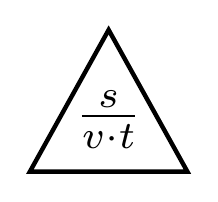
\begin{tikzpicture}[scale=2, every node/.style={scale=2}]
        \draw[ultra thick] (-0.5,-0.5) -- (0,-0.5) node[anchor=south, align=center] {\(\frac{s}{v \cdot t}\)} -- (0.5,-0.5) -- (0,0.4) -- cycle;
    \end{tikzpicture}
\end{figure*}

Denna kan användas genom att täcka för den sökta enheten med ett finger. och sedan kommer formel för den övertäcka enheten bli kvar. Sammanfattat gäller följande formler:
\begin{align*}
    s &= v \cdot t \\
    v &= \frac{s}{t} \\
    t &= \frac{s}{v} \\
\end{align*}

\section{Likformigt accelererande rörelse}
Om hastigheten inte längre är konstant är den enklaste nästa steg att accelerationen $a$ är konstant. då gäller följande formler:
\begin{align*}
    s &= \frac{at^2}{2} + v_0t + s_0 \\
    v &= at + v_0 
\end{align*}

\section{Allmän rörelse}
All rörelse kan beskrivas med hjälp av de ovanstående formlerna men man måste blanda in lite integral- och differentialkalkyl. För att uppnå denna fullständinga definition vill vi först tänka på rörelsens storheter som funktioner av tiden:
\begin{equation*}
    s(t) \text{ för sträcka, } v(t) \text{ för hastighet och } a(t) \text{ för accelration.}
\end{equation*}
Med detta kan vi sedan beräkna deras relation i alla möjliga fall. Här antar jag att du är bekant med tanken bakom integraler och derivator så här är snabbversionen av alla generella formler givet att $a(t)$ är linjärt:
\begin{align*}
    s(t) &= \frac{kt^3}{6} + \frac{a_0t^2}{2} + v_0t + s_0 \\
    v(t) &= \frac{kt^2}{2} + a_0t + v_0 \\
    a(t) &= kt + a_0
\end{align*}
eftersom
\begin{align*}
    v(t) &= s'(t) \\
    a(t) &= v'(t) = s''(t) \\
    s(t) &= \hyperref[def:indefint]{\int} {v(t)}\, dt = \iint{a(t)}\, dt\, dt
\end{align*}
(För fullständig härledning och teckenförklaring se bilaga \ref{derive:allmänrörelse}) Utifrån detta kan vi nu beräkna all rörelse bara vi vet formeln för en av storheterna. Om det inte finns en formel ska den hittas experimentellt eller så går det inte. Man kan sätta in valfri funktion för $a(t)$ och om man integrerar korrekt får man ändå rätt svar så detta är verkligen en allmän metod.

\section{Rörelsemängd}
Ett föremåls rörelsemängd är dess hastighet multiplicerat med dess massa och beteckans $p$. Formeln är: \[ p = mv\, \left[\mathrm{\frac{kg \cdot m}{s}  = kgm/s = N \cdot s}\right]\] Likt hastigheten är detta en vektor och har därför en riktning. Rörelsemängden skiljer sig från rörelseenergin $E_k$ eftersom $p \hyperref[def:propto]{\propto} v$ medan $E_k \propto v^2$.
\subsection{Stötar}
När två föremål krockar, dvs. stöter in i varandra så sker det ett utbyte av rörelsemängd. $p$ bevaras olika beroende på typen av stöt.
Se exempel nedan:
\begin{table*}[h]
    \centering
    \begin{tabular}{|c|c|c|}
        \hline
        Elastisk stöt          & Oelastiskt stöt             & fullständigt oelastisk stöt \\ \hline
        \begin{tikzpicture}
            \draw (0,0) -- (1,0);
        \end{tikzpicture}   &                             &                             \\ \hline
        Rörelseenergin bevaras & Rörelseenergin bevaras inte & Rörelseenergin bevaras inte \\ \hline
    \end{tabular}
\end{table*}
\subsubsection{Elastiskta stötar}
Vid s.k. \emph{elastiska stötar} så bevaras rörelseenergin. En elastisk stöt innebär att de två krockande föremålen inte fastnar i varandra utan förblir separata föremål. Generellt sett stöts de bort från varandra och åker åt olika håll efter stöten, dock inte alltid.

    \newpage
    \appendix
    \section{Härledningar}
    \label{appendix:härledning}
    \subsection{Teckenförklaring}
I denna sammanfattning använder jag vissa matematiska tecken som är ibland mer advancerade än bara de vi går igenom. Följande är deras definitioner:

\subsubsection*{Indefinit integral}
\label{def:indefint}
Tecknet $\int$ står för en \emph{indefinit integreal} när inga integrationsgränser är angivna. Detta motsvarar att hitta primitiv funktion till något så givet att \[f(x) = kx + m\] gäller att
\begin{equation*}
    F(x) = \int{f(x)}\, dx = \frac{kx^2}{2} + mx + C
\end{equation*}

Detta gäller för alla funktioner oavsett variabel, grad eller liknande man använder helt enkelt vanliga primitiva funktionsregler på lite mer effektivt sätt. Ja, man kan använda indefinit integral på prov enligt Mattias.

\subsubsection*{Proportionalitetstecken}
\label{def:propto}
Proportionalitetstecknet $\propto$ används för att visa att en variabel är proportionell mot någon annan variabel eller något uttryck. Givet proportionaliteten $y=kx$ kommer det se ut som \[y \propto x \text{ med en faktor k}\] 

\subsection{Allmän rörelse}
\label{derive:allmänrörelse}
Givet att funktionen $a(t) = kt + a_0$ där $a_0$ är en konstant startacceleration kommer nu härledningen till $s(t)$ från detta:
\begin{gather*}
    \begin{aligned}
        \centering
        a(t) &= kt + a_0 \\
        v(t) &= \int{a(t)}\, dt = \frac{kt^2}{2} + a_0t + C_1 & C_1 &= v_0 \\
        v(t) &= \frac{kt^2}{2} + a_0t + v_0 \\
        s(t) &= \int{v(t)}\, dt = \frac{kt^3}{6} + \frac{a_0t^2}{2} + v_0t + C_2 & C_2 &= s_0
    \end{aligned} \\
    \tcboxmath{s(t) = \frac{kt^3}{6} + \frac{a_0t^2}{2} + v_0t + s_0}
\end{gather*}
\noindent Här är \(a_0 = \text{acceleration från start, } v_0 = \text{hastighet från start och } s_0 = \text{den redan färdade sträckan från start}\). Alla integraler kan beräknas med reglerna från formelsamlingen.

\subsection{Lagen om rörelsemängdens bevarande}
\label{derive:conserverationmomentum}
Denna lag ger oss att efter en stöt kommer rörelsemängden i systemet alltid att bevaras. Föreställ dig att två föremål med massam $m_1$ och $m_2$ har hastigheterna $u_1$ och $u_2$. De krockar sedan elastiskt där föremål 1 verkar på föremål 2 med kraften $F_1$ medan föremål 2 verkar med kraften $F_2$. Sambandet mellan dessa krafter är
\begin{equation*}
    F_2 = -F_1 \: \text{enligt N III}
\end{equation*}
Föremålens krock pågår under en liten tid $\Delta t$. Impulsen som de båda påverkar varandra med blir då:
\begin{align*}
    \Delta p_1 &= F_2 \cdot \Delta t = m_1v_1 - m_1u_1 \\
    \Delta p_2 &= F_1 \cdot \Delta t = m_2v_2 - m_2u_2
\end{align*}
där $v_1$ och $v_2$ är hastigheterna efter krocken. Givet ovanstående kraftsamband får vi då:
\begin{align*}
    \Delta p_1 = -F_1 \cdot \Delta t &= -(F_1 \cdot \Delta t) = -\Delta p_2 \\
    \Delta p_1 &= -\Delta p_2 \\
    m_1v_1 - m_1u_1 &= -(m_2v_2 - m_2u_2) \\
    m_1v_1 - m_1u_1 &= -m_2v_2 + m_2u_2 \\
    m_1u_1 + m_2u_2 &= m_1v_1 + m_2v_2 \\
    p_{innan} &= p_{efter} \qed
\end{align*}
alltså konserveras rörelsemängden.

\subsection{Arkimedes princip}
\label{def:arkimedes}
Här följer en härledning för ett föremål med godtycklig volym och densitet givet arkimedes princip. Utifrån bilden kan vi se ett föremål med oregelbunden form som är ett vanligt prisma. Utifrån detta vet vi att $V = Ah$. Vi vet även den generella formeln för tryck i vätska: $P = \rho gh$. I detta fall är $h$ djupet i vätskan, jag vet att det är förvirrande med två $h$ men hellre detta än icke-standardiserade variabler. Detta ger oss följande iakttaglser:
\begin{equation*}
    P_1 = \rho gd \qquad P_2 = \rho g(d+h)
\end{equation*}
Efter detta inser man även att
\begin{equation*}
    |d+h| > |d| \implies P_2 > P_1
\end{equation*}
Vill vi få ut kraft ur ett tryck får vi att $F = PA$. Detta leder oss då till följande:
\begin{equation*}
    F_1 = P_1A \qquad F_2 = P_2A
\end{equation*}
sedan vet vi att
\begin{equation*}
    P_2 > P_1 \implies F_2 > F_1
\end{equation*}
För tydlighetens skulle är $F_2$ kraften som verkar uppåt på botten av föremålet på grund av vätsketrycket och $F_1$ är kraften som verkar nedåt på toppen av föremålet på grund av vätsketrycket. Utifrån dett kan vi logiskt inse att
\begin{gather*}
    \begin{aligned}
        F_L &= F_2 - F_1 \\
        F_L &= P_2A - P_1A \\
        F_L &= A(\rho g(d+h)) - A(\rho gd) \\
        F_L &= A\rho g((\cancel{d}+h)-\cancel{d}) \\
        F_L &= A\rho gh = Ah \cdot \rho g \qquad Ah = V
    \end{aligned} \\
    \tcboxmath{F_L = \rho gV \qed}
\end{gather*}
\begin{center}
    \begin{tikzpicture}[every path/.style={very thick}]
        %container
        \filldraw[color=cyan!80!blue, fill opacity=0.25] decorate [decoration={snake,amplitude=0.6mm,segment length=0.79cm}] {(-7,-0.3) -- ++ (14,0)} [rounded corners=5pt] -- ++(0,-6.7) -- ++(-14,0) [sharp corners] -- cycle;
        \draw[ultra thick, rounded corners=5pt, line cap=round] (-7,0) -- ++(0,-7) -- ++(14,0) -- ++(0,7);
        %shape
        \draw[line join=round] (-1,-1.5) .. controls (-0.8, -2) and (-0.4, -1.4) .. (0,-1.5) arc [start angle=85,delta angle=-200, radius=0.3cm] node [pos=0.4, anchor=east] {$A$} .. controls (-0.5,-1.9) .. (-1.3,-1.85) arc [start angle=272, delta angle=-250, radius=0.3cm] -- cycle;
        \draw[line join=round,yshift=-1.7cm] (-1,-1.5) .. controls (-0.8, -2) and (-0.4, -1.4) .. (0,-1.5) arc [start angle=85,delta angle=-200, radius=0.3cm] node [pos=0.4, anchor=east] {$A$} .. controls (-0.5,-1.9) .. (-1.3,-1.85) arc [start angle=272, delta angle=-250, radius=0.3cm] -- cycle;
        \draw[dashed, line cap=round] (-1.61,-1.5) -- ++(0,-1.7);
        \draw[dashed, line cap=round] (0.27, -1.8) -- ++(0,-1.7);
        %height
        \draw[decorate, decoration={calligraphic brace,amplitude=2mm}, xshift=0.1cm] (0.27, -1.8) -- ++(0,-1.7) node[pos=0.5, anchor=west, right=2pt] {$h$};
        \draw[decorate, decoration={calligraphic brace,amplitude=2mm}, xshift=0.1cm] (0.27, -0.23) -- ++(0,-1.53) node[pos=0.5, anchor=west, right=2pt] {$d$};
    \end{tikzpicture}
\end{center}

    \section{Exempel}
    \label{appendix:exempel}
\end{document}